%%% Local Variables:
%%% mode: latex
%%% TeX-master: main
%%% End:


\marginpar{\scriptsize cache}\exercise~A Tabela~\ref{tab:refs} contem uma lista de
referências para endereços de memória de 5 bits.

\begin{table}[h]
\centering
\begin{tabular}{|l|l|}\hline
  \bf a. & 0, 31, 12, 7, 31, 13, 12, 31, 7, 31, 7, 12 \\\hline
  \bf b. & 1, 17, 1, 17, 5, 25, 29, 1, 25, 29, 17, 1 \\\hline
\end{tabular}
\caption{Tabela de referências para duas requisições de endereços para
  a memória cache.}
\label{tab:refs}
\end{table}

Para cada uma das referências da Tabela~\ref{tab:refs}, realizar os
{\bf mapeamentos direto (itens a, b) e associativo em quatro (somente
item a) e duas vias (somente item b)} de uma cache com {\bf 8}
blocos. Também listar se cada referência requisitada apresenta {\it
cache hit/miss\/} calculando a taxa de ausência de endereços. Assumir
que inicialmente a cache está vazia.

Se houver necessidade de substituição de blocos na cache, utilize o
algoritmo LRU ({\em Last Recently Used} -- último recentemente usado)
para definir qual endereço será substituído na memória cache.

\exercise~Descreva as seguintes políticas de escrita da memória cache
para a memória principal:

\begin{itemize}
\item {\em write-buffer};
\item {\em write-back}.
\end{itemize}

 \marginpar{\scriptsize cache}\exercise~A Figura~\ref{fig:incr}~mostra a
sequência de execução de instruções MIPS para incrementar o segundo
elemento {\tt V[1]} do vetor {\tt V[0..N-1]}. O endereço do início do
vetor {\tt V[]} está armazenado no registrador {\tt \$t0}, e o
conteúdo de {\tt V[1]} armazenado no registrador {\tt \$s0}. Supondo
que a requisição do endereço contido em {\tt \$t0} não esteja
disponível na memória cache, ou seja, que a primeira instrução obtenha
{\em cache miss}, indique o valor dos bits de validade e de sujeira ao
final dos tempos $2, 4, 6$, para a entrada na tabela de referências da
cache referente ao endereço contido em {\tt \$t0}.

\begin{figure}[h]
\centering
\begin{ganttchart}[hgrid, vgrid]{1}{7}
\gantttitlelist{1,...,7}{1} \\
\ganttbar{\tt\scriptsize lw~\$s0,4(\$t0)}{1}{2}\\
\ganttbar{\tt\scriptsize addi~\$s0,\$s0,1}{3}{3}\\
\ganttbar{\tt\scriptsize sw~\$s0,4(\$t0)}{5}{6}
\end{ganttchart}
\caption{Sequência de execução de instruções MIPS para incrementar o
conteúdo do registrador {\tt \$s0}.}
\label{fig:incr}
\end{figure}

\marginpar{\scriptsize memória virtual}\exercise~Com relação ao exercício
anterior, se o endereço requisitado já estiver na memória principal
antes da execução da primeira instrução, qual será o valor do bit de
sujeira na tabela de páginas após a execução das 3 instruções.


\marginpar{\em\small cache miss}\exercise~Assuma uma cache com
mapeamento associativo em $2$ conjuntos com 4 blocos, como demonstrado
na Tabela~\ref{tab:miss} para a sequência de endereços ``0, 1, 2, 3, 4''.

\begin{table}[ht]
\scriptsize
\centering
\begin{tabular}[ht]{p{3cm}cp{1cm}p{1cm}p{1cm}p{1cm}p{1cm}}\hline
Endereço do bloco de memória acessado& \em hit/miss & bloco trocado &
conjunto 0 & conjunto 0 & conjunto 1 & conjunto 1\\\hline
0 & \em miss & & M(0) & & & \\
1 & \em miss & & M(0) & & M(1) & \\
2 & \em miss & & M(0) & M(2) & M(1) & \\
3 & \em miss & & M(0) & M(2) & M(1) & M(3)\\
4 & \em miss & 0 & M(4) & M(2) & M(1) & M(3)\\
$\ldots$ &  & & & & & \\\hline
\end{tabular}
\caption{Sequências de requisições de endereços para a memória cache.}
\label{tab:miss}
\end{table}

Continue a construção da Tabela~\ref{tab:miss} para as seguintes
requisições de endereços:

\begin{enumerate}[a)]
\item $0,2,4,0,2,4,0,2,4$;
\item $0,2,4,2,0,2,4,0,2$.
\end{enumerate}


\marginpar{\scriptsize memória virtual}\exercise~Explique quais as
mudanças que ocorrem na TLB e tabela de páginas mostradas a seguir,
com a requisição das páginas ``11'' e ``5''.

\bigskip
\begin{minipage}[h]{.5\linewidth}
\centering
\scriptsize
{\bf TLB}\\
\begin{tabular}[h]{c|c|p{3cm}}\hline
Validade & \em Tag & número do endereço físico da página\\\hline
1 & 11 & 12\\
1 & 7 & 4 \\
1 & 3 & 6 \\
0 & 4 & 9 \\\hline
\end{tabular}
\end{minipage}
\begin{minipage}[h]{.5\linewidth}
\centering
\scriptsize
{\bf Tabela de páginas}\\
\begin{tabular}[h]{c|p{3cm}}\hline
Validade & endereço físico na memória ou disco \\\hline
1 & 5 \\
0 & 4095 \\
0 & 31272 \\
1 & 6 \\
1 & 9 \\
1 & 11 \\
0 & 19136\\
1 & 4 \\
0 & 48480\\
0 & 38110 \\
1 & 3\\
1 & 12 \\\hline
\end{tabular}
\end{minipage}

\bigskip
\noindent Responda também quais endereços pertencentes ao programa
ainda não estão armazenados na memória principal, e se houvesse
requisições para estes endereços de disco, qual seria a sequência
de endereços atendida.

\end{document}

\paragraph{Exercício 0.}
A listagem a seguir contem uma lista de referências para endereços
de memória DRAM de {\bf 5} bits.

\begin{center}
  \tt
  0, 16, 8, 0, 0, 4, 3, 12, 3, 11, 12, 21, 21, 22, 28, 6, 4 \\
\end{center}

Para cada uma das referências, realizar os seguintes mapeamentos:

\begin{itemize}
\item Mapeamento associativo direto;
\item {\bf Mapeamento associativo em conjunto com duas vias}, utilizando o
  algoritmo {\bf LRU}\footnote{Último usado recentemente} para
  reposição dos blocos na memória cache (SRAM);
\item {\bf Mapeamento associativo em conjunto com duas
  vias}, utilizando o algoritmo {\bf aleatório }
  para reposição dos blocos na memória cache (SRAM);
\item {\bf Sem mapeamento}, utilizando o algoritmo {\bf LRU} para
  reposição dos blocos na memória cache (SRAM);
\item {\bf Sem mapeamento}, utilizando o algoritmo {\bf aleatório } para
  reposição dos blocos na memória cache (SRAM);
\end{itemize}


\newcounter{dramaddr}\setcounter{dramaddr}{0}
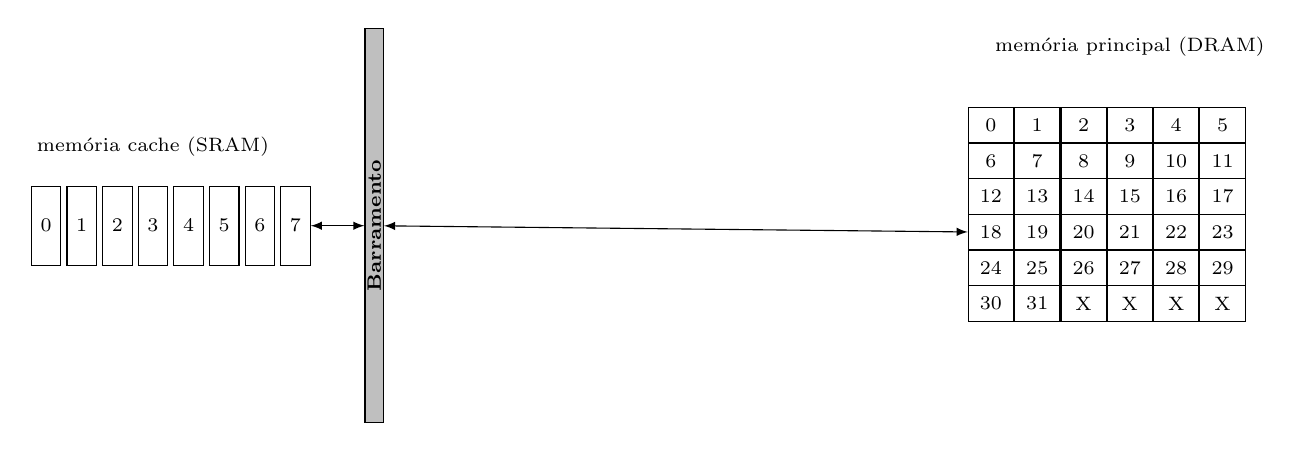
\begin{tikzpicture}[font=\scriptsize]
  \foreach \x in {0,...,7} {
    \node[minimum height=1cm, draw] (c\x) at (\x/2.21,0) [below] {\scriptsize \x};
  }
  \node [minimum height=5cm, right of=c7, fill=lightgray, draw] (bus)
  {};
  \node[rotate=90] at (bus) {\bf Barramento};
  \node [above of=c3] {memória cache (SRAM)};

%  \foreach \x in {1,3,5,7} {
 %   \draw (c\x)+(0.0,0cm) -- (c\x)+(0.0cm,4cm);
 % }

  \foreach \y in {0,...,5} {
    \foreach \x in {0,...,5} {
      \def\addr{\arabic{dramaddr}}
     
      \node[minimum height=.45cm, minimum width=.575cm, draw] (m\x\y) at
      (12+\x/1.7,1-\y/2.21) [below] {\scriptsize \ifnum\addr<32 \addr
      \else X \fi};
      \addtocounter{dramaddr}{1}
    }
  }

    \path[<->,>=latex,draw] (c7) -- (bus);
    \path[<->,>=latex,draw] (bus) -- (m03);
\node [above of=m30] {memória principal (DRAM)};
\end{tikzpicture}

\subsection*{Solução}

\subsubsection*{Mapeamento associativo direto}


\begin{minipage}{.5\textwidth}
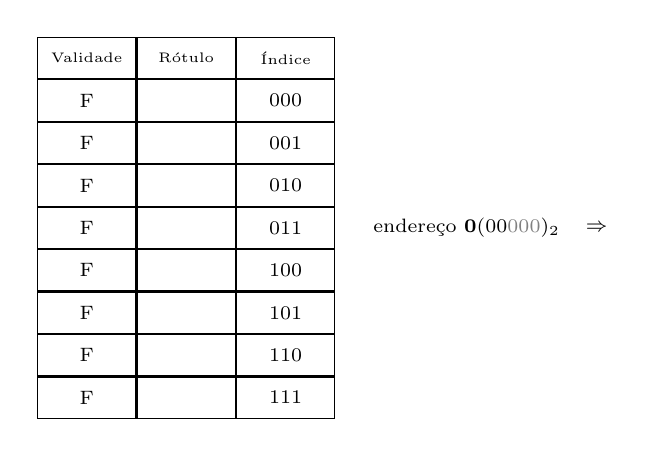
\begin{tikzpicture}[mat/.style={minimum width=1.25cm, minimum
    height=.525cm, draw}, every node/.style={font=\scriptsize}]
  \pgfsetmatrixcolumnsep{1mm}
  \pgfmatrix{rectangle}{center}{mymatrix}
  {\pgfusepath{}}{\pgfpointorigin}{\let\&=\pgfmatrixnextcell}
  {
    \node[mat] {\tiny Validade}; \&[-1mm] \node[mat]{\tiny Rótulo}; \&[-1mm]
    \node[mat] {\tiny Índice}; \\
    \node[mat] {F}; \& \node[mat]{}; \&  \node[mat] {000}; \\
    \node[mat] {F}; \&  \node[mat]{}; \&  \node[mat] {001}; \\
    \node[mat] {F}; \& \node[mat]{}; \&  \node[mat] {010}; \\
    \node[mat] {F}; \&  \node[mat]{}; \&  \node[mat] (b0) {011}; \\
    \node[mat] {F}; \& \node[mat]{}; \&  \node[mat] {100}; \\
    \node[mat] {F}; \&  \node[mat]{}; \&  \node[mat] {101}; \\
    \node[mat] {F}; \& \node[mat]{}; \&  \node[mat] {110}; \\
    \node[mat] {F}; \&  \node[mat]{}; \&  \node[mat] {111}; \\
  }

  \node (r0) [right of=b0, xshift=1.25cm] {\lw\ endereço {\bf
      0}(00{\color{gray} 000})$_2$};
  \node (s0) [right of=r0, xshift=.7cm] {$\Rightarrow$};
  \node  [above of=s0] {{\it \miss}};
\end{tikzpicture}
\end{minipage}
\begin{minipage}{.5\textwidth}
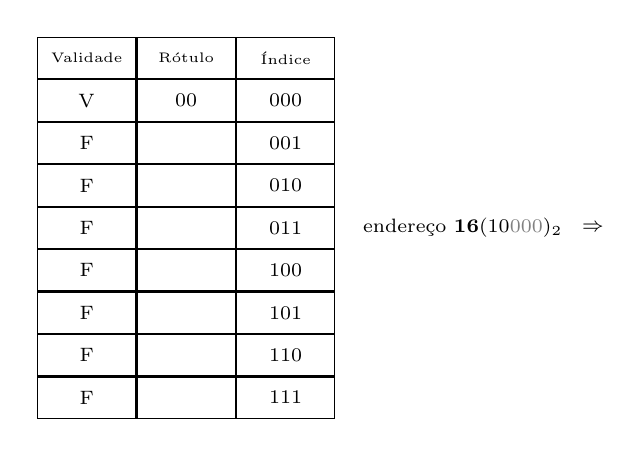
\begin{tikzpicture}[mat/.style={minimum width=1.25cm, minimum
    height=.525cm, draw}, every node/.style={font=\scriptsize}]
  \pgfsetmatrixcolumnsep{1mm}
  \pgfmatrix{rectangle}{center}{mymatrix}
  {\pgfusepath{}}{\pgfpointorigin}{\let\&=\pgfmatrixnextcell}
  {
    \node[mat] {\tiny Validade}; \&[-1mm] \node[mat]{\tiny Rótulo}; \&[-1mm]
    \node[mat] {\tiny Índice}; \\
    \node[mat] {V}; \& \node[mat]{00}; \&  \node[mat] {000}; \\
    \node[mat] {F}; \&  \node[mat]{}; \&  \node[mat] {001}; \\
    \node[mat] {F}; \& \node[mat]{}; \&  \node[mat] {010}; \\
    \node[mat] {F}; \&  \node[mat]{}; \&  \node[mat] (b0) {011}; \\
    \node[mat] {F}; \& \node[mat]{}; \&  \node[mat] {100}; \\
    \node[mat] {F}; \&  \node[mat]{}; \&  \node[mat] {101}; \\
    \node[mat] {F}; \& \node[mat]{}; \&  \node[mat] {110}; \\
    \node[mat] {F}; \&  \node[mat]{}; \&  \node[mat] {111}; \\
  }

  \node (r0) [right of=b0, xshift=1.2cm] {\lw\ endereço {\bf 16}(10{\color{gray} 000})$_2$};
  \node (s1) [right of=r0, xshift=.7cm] {$\Rightarrow$};
  \node  [above of=s1] {{\it \miss}};
\end{tikzpicture}
\end{minipage}


\noindent\begin{minipage}{.5\textwidth}
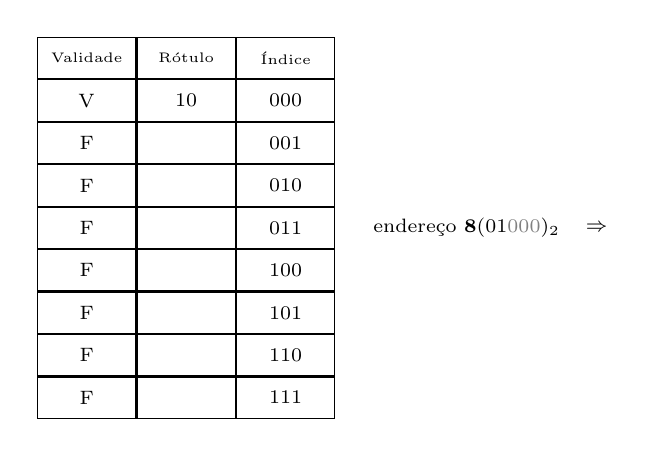
\begin{tikzpicture}[mat/.style={minimum width=1.25cm, minimum
    height=.525cm, draw}, every node/.style={font=\scriptsize}]
  \pgfsetmatrixcolumnsep{1mm}
  \pgfmatrix{rectangle}{center}{mymatrix}
  {\pgfusepath{}}{\pgfpointorigin}{\let\&=\pgfmatrixnextcell}
  {
    \node[mat] {\tiny Validade}; \&[-1mm] \node[mat]{\tiny Rótulo}; \&[-1mm]
    \node[mat] {\tiny Índice}; \\
    \node[mat] {V}; \& \node[mat]{10}; \&  \node[mat] {000}; \\
    \node[mat] {F}; \&  \node[mat]{}; \&  \node[mat] {001}; \\
    \node[mat] {F}; \& \node[mat]{}; \&  \node[mat] {010}; \\
    \node[mat] {F}; \&  \node[mat]{}; \&  \node[mat] (b0) {011}; \\
    \node[mat] {F}; \& \node[mat]{}; \&  \node[mat] {100}; \\
    \node[mat] {F}; \&  \node[mat]{}; \&  \node[mat] {101}; \\
    \node[mat] {F}; \& \node[mat]{}; \&  \node[mat] {110}; \\
    \node[mat] {F}; \&  \node[mat]{}; \&  \node[mat] {111}; \\
  }

  \node (r0) [right of=b0, xshift=1.25cm] {\lw\ endereço {\bf
      8}(01{\color{gray} 000})$_2$};
  \node (s0) [right of=r0, xshift=.7cm] {$\Rightarrow$};
  \node  [above of=s0] {{\it \miss}};
\end{tikzpicture}
\end{minipage}
\begin{minipage}{.5\textwidth}
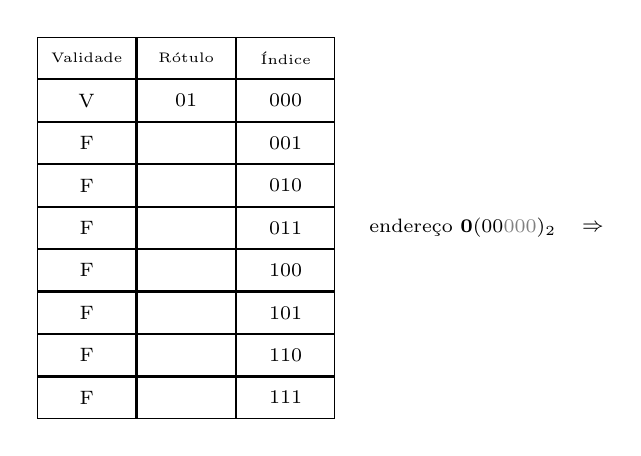
\begin{tikzpicture}[mat/.style={minimum width=1.25cm, minimum
    height=.525cm, draw}, every node/.style={font=\scriptsize}]
  \pgfsetmatrixcolumnsep{1mm}
  \pgfmatrix{rectangle}{center}{mymatrix}
  {\pgfusepath{}}{\pgfpointorigin}{\let\&=\pgfmatrixnextcell}
  {
    \node[mat] {\tiny Validade}; \&[-1mm] \node[mat]{\tiny Rótulo}; \&[-1mm]
    \node[mat] {\tiny Índice}; \\
    \node[mat] {V}; \& \node[mat]{01}; \&  \node[mat] {000}; \\
    \node[mat] {F}; \&  \node[mat]{}; \&  \node[mat] {001}; \\
    \node[mat] {F}; \& \node[mat]{}; \&  \node[mat] {010}; \\
    \node[mat] {F}; \&  \node[mat]{}; \&  \node[mat] (b0) {011}; \\
    \node[mat] {F}; \& \node[mat]{}; \&  \node[mat] {100}; \\
    \node[mat] {F}; \&  \node[mat]{}; \&  \node[mat] {101}; \\
    \node[mat] {F}; \& \node[mat]{}; \&  \node[mat] {110}; \\
    \node[mat] {F}; \&  \node[mat]{}; \&  \node[mat] {111}; \\
  }

  \node (r0) [right of=b0, xshift=1.2cm] {\lw\ endereço {\bf 0}(00{\color{gray} 000})$_2$};
  \node (s1) [right of=r0, xshift=.7cm] {$\Rightarrow$};
  \node  [above of=s1] {{\it \miss}};
\end{tikzpicture}
\end{minipage}


\noindent\begin{minipage}{.5\textwidth}
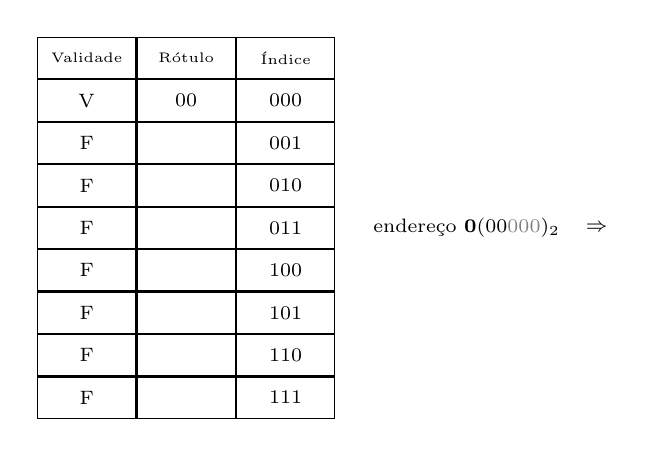
\begin{tikzpicture}[mat/.style={minimum width=1.25cm, minimum
    height=.525cm, draw}, every node/.style={font=\scriptsize}]
  \pgfsetmatrixcolumnsep{1mm}
  \pgfmatrix{rectangle}{center}{mymatrix}
  {\pgfusepath{}}{\pgfpointorigin}{\let\&=\pgfmatrixnextcell}
  {
    \node[mat] {\tiny Validade}; \&[-1mm] \node[mat]{\tiny Rótulo}; \&[-1mm]
    \node[mat] {\tiny Índice}; \\
    \node[mat] {V}; \& \node[mat]{00}; \&  \node[mat] {000}; \\
    \node[mat] {F}; \&  \node[mat]{}; \&  \node[mat] {001}; \\
    \node[mat] {F}; \& \node[mat]{}; \&  \node[mat] {010}; \\
    \node[mat] {F}; \&  \node[mat]{}; \&  \node[mat] (b0) {011}; \\
    \node[mat] {F}; \& \node[mat]{}; \&  \node[mat] {100}; \\
    \node[mat] {F}; \&  \node[mat]{}; \&  \node[mat] {101}; \\
    \node[mat] {F}; \& \node[mat]{}; \&  \node[mat] {110}; \\
    \node[mat] {F}; \&  \node[mat]{}; \&  \node[mat] {111}; \\
  }

  \node (r0) [right of=b0, xshift=1.25cm] {\lw\ endereço {\bf
      0}(00{\color{gray} 000})$_2$};
  \node (s0) [right of=r0, xshift=.7cm] {$\Rightarrow$};
  \node  [above of=s0] {{\it \HIT}};
\end{tikzpicture}
\end{minipage}
\begin{minipage}{.5\textwidth}
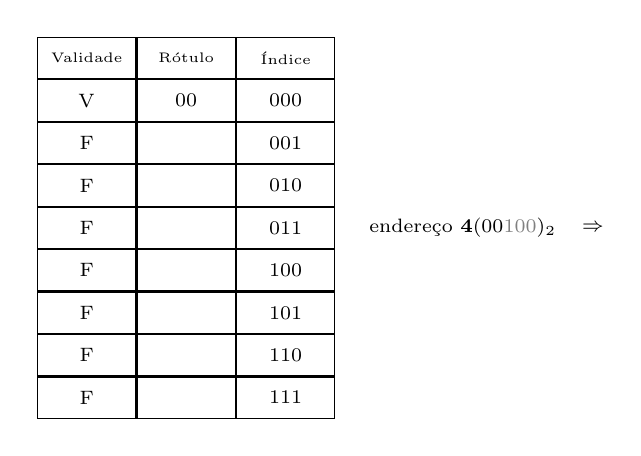
\begin{tikzpicture}[mat/.style={minimum width=1.25cm, minimum
    height=.525cm, draw}, every node/.style={font=\scriptsize}]
  \pgfsetmatrixcolumnsep{1mm}
  \pgfmatrix{rectangle}{center}{mymatrix}
  {\pgfusepath{}}{\pgfpointorigin}{\let\&=\pgfmatrixnextcell}
  {
    \node[mat] {\tiny Validade}; \&[-1mm] \node[mat]{\tiny Rótulo}; \&[-1mm]
    \node[mat] {\tiny Índice}; \\
    \node[mat] {V}; \& \node[mat]{00}; \&  \node[mat] {000}; \\
    \node[mat] {F}; \&  \node[mat]{}; \&  \node[mat] {001}; \\
    \node[mat] {F}; \& \node[mat]{}; \&  \node[mat] {010}; \\
    \node[mat] {F}; \&  \node[mat]{}; \&  \node[mat] (b0) {011}; \\
    \node[mat] {F}; \& \node[mat]{}; \&  \node[mat] {100}; \\
    \node[mat] {F}; \&  \node[mat]{}; \&  \node[mat] {101}; \\
    \node[mat] {F}; \& \node[mat]{}; \&  \node[mat] {110}; \\
    \node[mat] {F}; \&  \node[mat]{}; \&  \node[mat] {111}; \\
  }

  \node (r0) [right of=b0, xshift=1.2cm] {\lw\ endereço {\bf 4}(00{\color{gray} 100})$_2$};
  \node (s1) [right of=r0, xshift=.7cm] {$\Rightarrow$};
  \node  [above of=s1] {{\it \miss}};
\end{tikzpicture}
\end{minipage}


\noindent\begin{minipage}{.5\textwidth}
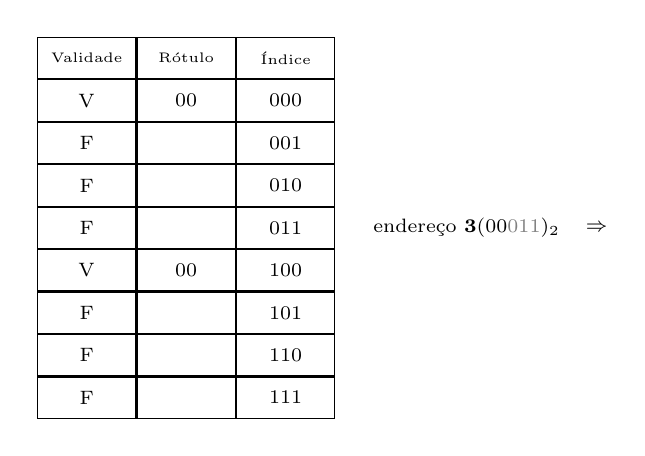
\begin{tikzpicture}[mat/.style={minimum width=1.25cm, minimum
    height=.525cm, draw}, every node/.style={font=\scriptsize}]
  \pgfsetmatrixcolumnsep{1mm}
  \pgfmatrix{rectangle}{center}{mymatrix}
  {\pgfusepath{}}{\pgfpointorigin}{\let\&=\pgfmatrixnextcell}
  {
    \node[mat] {\tiny Validade}; \&[-1mm] \node[mat]{\tiny Rótulo}; \&[-1mm]
    \node[mat] {\tiny Índice}; \\
    \node[mat] {V}; \& \node[mat]{00}; \&  \node[mat] {000}; \\
    \node[mat] {F}; \&  \node[mat]{}; \&  \node[mat] {001}; \\
    \node[mat] {F}; \& \node[mat]{}; \&  \node[mat] {010}; \\
    \node[mat] {F}; \&  \node[mat]{}; \&  \node[mat] (b0) {011}; \\
    \node[mat] {V}; \& \node[mat]{00}; \&  \node[mat] {100}; \\
    \node[mat] {F}; \&  \node[mat]{}; \&  \node[mat] {101}; \\
    \node[mat] {F}; \& \node[mat]{}; \&  \node[mat] {110}; \\
    \node[mat] {F}; \&  \node[mat]{}; \&  \node[mat] {111}; \\
  }

  \node (r0) [right of=b0, xshift=1.25cm] {\lw\ endereço {\bf
      3}(00{\color{gray} 011})$_2$};
  \node (s0) [right of=r0, xshift=.7cm] {$\Rightarrow$};
  \node  [above of=s0] {{\it \miss}};
\end{tikzpicture}
\end{minipage}
\begin{minipage}{.5\textwidth}
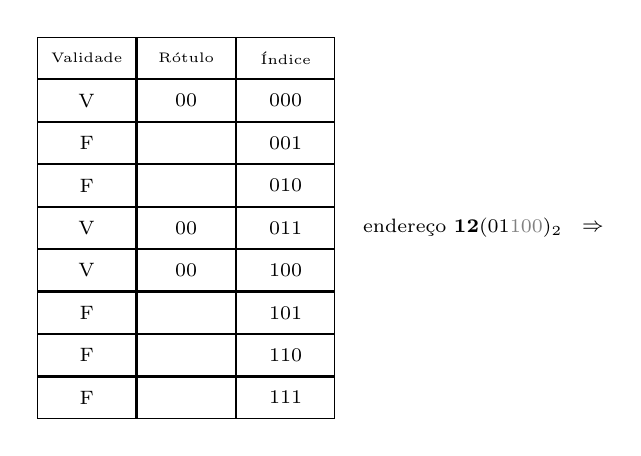
\begin{tikzpicture}[mat/.style={minimum width=1.25cm, minimum
    height=.525cm, draw}, every node/.style={font=\scriptsize}]
  \pgfsetmatrixcolumnsep{1mm}
  \pgfmatrix{rectangle}{center}{mymatrix}
  {\pgfusepath{}}{\pgfpointorigin}{\let\&=\pgfmatrixnextcell}
  {
    \node[mat] {\tiny Validade}; \&[-1mm] \node[mat]{\tiny Rótulo}; \&[-1mm]
    \node[mat] {\tiny Índice}; \\
    \node[mat] {V}; \& \node[mat]{00}; \&  \node[mat] {000}; \\
    \node[mat] {F}; \&  \node[mat]{}; \&  \node[mat] {001}; \\
    \node[mat] {F}; \& \node[mat]{}; \&  \node[mat] {010}; \\
    \node[mat] {V}; \&  \node[mat]{00}; \&  \node[mat] (b0) {011}; \\
    \node[mat] {V}; \& \node[mat]{00}; \&  \node[mat] {100}; \\
    \node[mat] {F}; \&  \node[mat]{}; \&  \node[mat] {101}; \\
    \node[mat] {F}; \& \node[mat]{}; \&  \node[mat] {110}; \\
    \node[mat] {F}; \&  \node[mat]{}; \&  \node[mat] {111}; \\
  }

  \node (r0) [right of=b0, xshift=1.2cm] {\lw\ endereço {\bf 12}(01{\color{gray} 100})$_2$};
  \node (s1) [right of=r0, xshift=.7cm] {$\Rightarrow$};
  \node  [above of=s1] {{\it \miss}};
\end{tikzpicture}
\end{minipage}


\noindent\begin{minipage}{.5\textwidth}
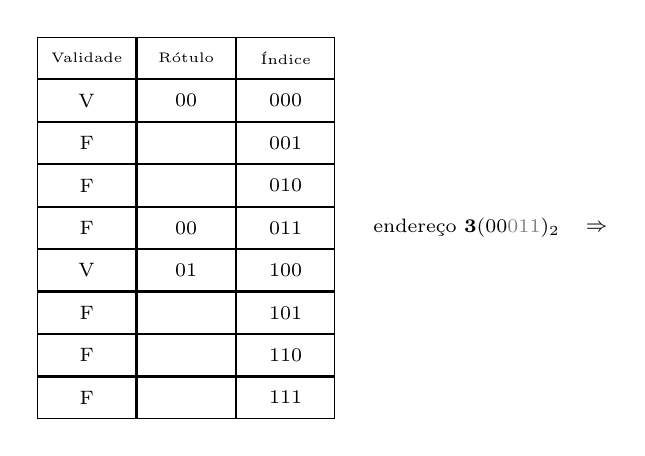
\begin{tikzpicture}[mat/.style={minimum width=1.25cm, minimum
    height=.525cm, draw}, every node/.style={font=\scriptsize}]
  \pgfsetmatrixcolumnsep{1mm}
  \pgfmatrix{rectangle}{center}{mymatrix}
  {\pgfusepath{}}{\pgfpointorigin}{\let\&=\pgfmatrixnextcell}
  {
    \node[mat] {\tiny Validade}; \&[-1mm] \node[mat]{\tiny Rótulo}; \&[-1mm]
    \node[mat] {\tiny Índice}; \\
    \node[mat] {V}; \& \node[mat]{00}; \&  \node[mat] {000}; \\
    \node[mat] {F}; \&  \node[mat]{}; \&  \node[mat] {001}; \\
    \node[mat] {F}; \& \node[mat]{}; \&  \node[mat] {010}; \\
    \node[mat] {F}; \&  \node[mat]{00}; \&  \node[mat] (b0) {011}; \\
    \node[mat] {V}; \& \node[mat]{01}; \&  \node[mat] {100}; \\
    \node[mat] {F}; \&  \node[mat]{}; \&  \node[mat] {101}; \\
    \node[mat] {F}; \& \node[mat]{}; \&  \node[mat] {110}; \\
    \node[mat] {F}; \&  \node[mat]{}; \&  \node[mat] {111}; \\
  }

  \node (r0) [right of=b0, xshift=1.25cm] {\lw\ endereço {\bf
      3}(00{\color{gray} 011})$_2$};
  \node (s0) [right of=r0, xshift=.7cm] {$\Rightarrow$};
  \node  [above of=s0] {{\it \HIT}};
\end{tikzpicture}
\end{minipage}
\begin{minipage}{.5\textwidth}
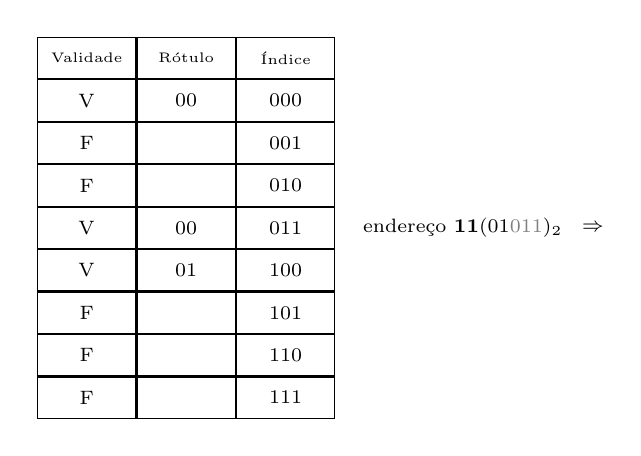
\begin{tikzpicture}[mat/.style={minimum width=1.25cm, minimum
    height=.525cm, draw}, every node/.style={font=\scriptsize}]
  \pgfsetmatrixcolumnsep{1mm}
  \pgfmatrix{rectangle}{center}{mymatrix}
  {\pgfusepath{}}{\pgfpointorigin}{\let\&=\pgfmatrixnextcell}
  {
    \node[mat] {\tiny Validade}; \&[-1mm] \node[mat]{\tiny Rótulo}; \&[-1mm]
    \node[mat] {\tiny Índice}; \\
    \node[mat] {V}; \& \node[mat]{00}; \&  \node[mat] {000}; \\
    \node[mat] {F}; \&  \node[mat]{}; \&  \node[mat] {001}; \\
    \node[mat] {F}; \& \node[mat]{}; \&  \node[mat] {010}; \\
    \node[mat] {V}; \&  \node[mat]{00}; \&  \node[mat] (b0) {011}; \\
    \node[mat] {V}; \& \node[mat]{01}; \&  \node[mat] {100}; \\
    \node[mat] {F}; \&  \node[mat]{}; \&  \node[mat] {101}; \\
    \node[mat] {F}; \& \node[mat]{}; \&  \node[mat] {110}; \\
    \node[mat] {F}; \&  \node[mat]{}; \&  \node[mat] {111}; \\
  }

  \node (r0) [right of=b0, xshift=1.2cm] {\lw\ endereço {\bf 11}(01{\color{gray} 011})$_2$};
  \node (s1) [right of=r0, xshift=.7cm] {$\Rightarrow$};
  \node  [above of=s1] {{\it \miss}};
\end{tikzpicture}
\end{minipage}

\noindent\begin{minipage}{.5\textwidth}
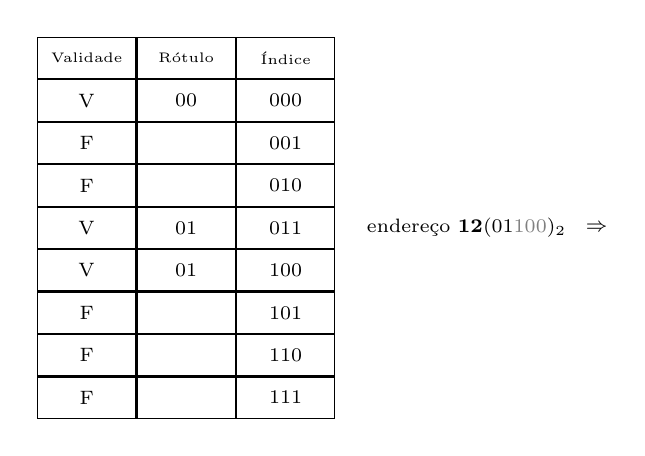
\begin{tikzpicture}[mat/.style={minimum width=1.25cm, minimum
    height=.525cm, draw}, every node/.style={font=\scriptsize}]
  \pgfsetmatrixcolumnsep{1mm}
  \pgfmatrix{rectangle}{center}{mymatrix}
  {\pgfusepath{}}{\pgfpointorigin}{\let\&=\pgfmatrixnextcell}
  {
    \node[mat] {\tiny Validade}; \&[-1mm] \node[mat]{\tiny Rótulo}; \&[-1mm]
    \node[mat] {\tiny Índice}; \\
    \node[mat] {V}; \& \node[mat]{00}; \&  \node[mat] {000}; \\
    \node[mat] {F}; \&  \node[mat]{}; \&  \node[mat] {001}; \\
    \node[mat] {F}; \& \node[mat]{}; \&  \node[mat] {010}; \\
    \node[mat] {V}; \&  \node[mat]{01}; \&  \node[mat] (b0) {011}; \\
    \node[mat] {V}; \& \node[mat]{01}; \&  \node[mat] {100}; \\
    \node[mat] {F}; \&  \node[mat]{}; \&  \node[mat] {101}; \\
    \node[mat] {F}; \& \node[mat]{}; \&  \node[mat] {110}; \\
    \node[mat] {F}; \&  \node[mat]{}; \&  \node[mat] {111}; \\
  }

  \node (r0) [right of=b0, xshift=1.25cm] {\lw\ endereço {\bf
      12}(01{\color{gray} 100})$_2$};
  \node (s0) [right of=r0, xshift=.7cm] {$\Rightarrow$};
  \node  [above of=s0] {{\it \HIT}};
\end{tikzpicture}
\end{minipage}
\begin{minipage}{.5\textwidth}
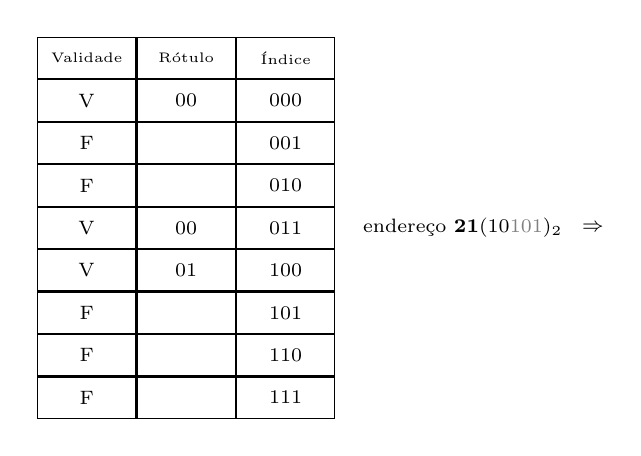
\begin{tikzpicture}[mat/.style={minimum width=1.25cm, minimum
    height=.525cm, draw}, every node/.style={font=\scriptsize}]
  \pgfsetmatrixcolumnsep{1mm}
  \pgfmatrix{rectangle}{center}{mymatrix}
  {\pgfusepath{}}{\pgfpointorigin}{\let\&=\pgfmatrixnextcell}
  {
    \node[mat] {\tiny Validade}; \&[-1mm] \node[mat]{\tiny Rótulo}; \&[-1mm]
    \node[mat] {\tiny Índice}; \\
    \node[mat] {V}; \& \node[mat]{00}; \&  \node[mat] {000}; \\
    \node[mat] {F}; \&  \node[mat]{}; \&  \node[mat] {001}; \\
    \node[mat] {F}; \& \node[mat]{}; \&  \node[mat] {010}; \\
    \node[mat] {V}; \&  \node[mat]{00}; \&  \node[mat] (b0) {011}; \\
    \node[mat] {V}; \& \node[mat]{01}; \&  \node[mat] {100}; \\
    \node[mat] {F}; \&  \node[mat]{}; \&  \node[mat] {101}; \\
    \node[mat] {F}; \& \node[mat]{}; \&  \node[mat] {110}; \\
    \node[mat] {F}; \&  \node[mat]{}; \&  \node[mat] {111}; \\
  }

  \node (r0) [right of=b0, xshift=1.2cm] {\lw\ endereço {\bf 21}(10{\color{gray} 101})$_2$};
  \node (s1) [right of=r0, xshift=.7cm] {$\Rightarrow$};
  \node  [above of=s1] {{\it \miss}};
\end{tikzpicture}
\end{minipage}


\noindent\begin{minipage}{.5\textwidth}
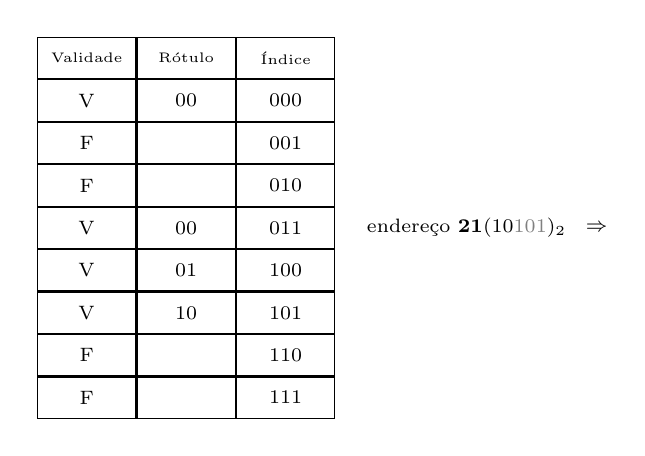
\begin{tikzpicture}[mat/.style={minimum width=1.25cm, minimum
    height=.525cm, draw}, every node/.style={font=\scriptsize}]
  \pgfsetmatrixcolumnsep{1mm}
  \pgfmatrix{rectangle}{center}{mymatrix}
  {\pgfusepath{}}{\pgfpointorigin}{\let\&=\pgfmatrixnextcell}
  {
    \node[mat] {\tiny Validade}; \&[-1mm] \node[mat]{\tiny Rótulo}; \&[-1mm]
    \node[mat] {\tiny Índice}; \\
    \node[mat] {V}; \& \node[mat]{00}; \&  \node[mat] {000}; \\
    \node[mat] {F}; \&  \node[mat]{}; \&  \node[mat] {001}; \\
    \node[mat] {F}; \& \node[mat]{}; \&  \node[mat] {010}; \\
    \node[mat] {V}; \&  \node[mat]{00}; \&  \node[mat] (b0) {011}; \\
    \node[mat] {V}; \& \node[mat]{01}; \&  \node[mat] {100}; \\
    \node[mat] {V}; \&  \node[mat]{10}; \&  \node[mat] {101}; \\
    \node[mat] {F}; \& \node[mat]{}; \&  \node[mat] {110}; \\
    \node[mat] {F}; \&  \node[mat]{}; \&  \node[mat] {111}; \\
  }

  \node (r0) [right of=b0, xshift=1.25cm] {\lw\ endereço {\bf
      21}(10{\color{gray} 101})$_2$};
  \node (s0) [right of=r0, xshift=.7cm] {$\Rightarrow$};
  \node  [above of=s0] {{\it \HIT}};
\end{tikzpicture}
\end{minipage}
\begin{minipage}{.5\textwidth}
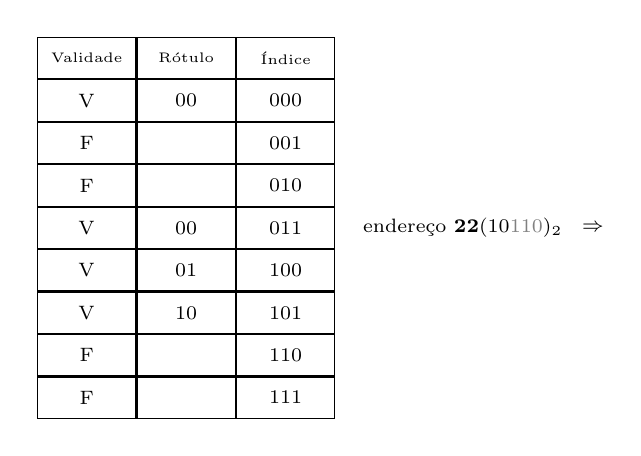
\begin{tikzpicture}[mat/.style={minimum width=1.25cm, minimum
    height=.525cm, draw}, every node/.style={font=\scriptsize}]
  \pgfsetmatrixcolumnsep{1mm}
  \pgfmatrix{rectangle}{center}{mymatrix}
  {\pgfusepath{}}{\pgfpointorigin}{\let\&=\pgfmatrixnextcell}
  {
    \node[mat] {\tiny Validade}; \&[-1mm] \node[mat]{\tiny Rótulo}; \&[-1mm]
    \node[mat] {\tiny Índice}; \\
    \node[mat] {V}; \& \node[mat]{00}; \&  \node[mat] {000}; \\
    \node[mat] {F}; \&  \node[mat]{}; \&  \node[mat] {001}; \\
    \node[mat] {F}; \& \node[mat]{}; \&  \node[mat] {010}; \\
    \node[mat] {V}; \&  \node[mat]{00}; \&  \node[mat] (b0) {011}; \\
    \node[mat] {V}; \& \node[mat]{01}; \&  \node[mat] {100}; \\
    \node[mat] {V}; \&  \node[mat]{10}; \&  \node[mat] {101}; \\
    \node[mat] {F}; \& \node[mat]{}; \&  \node[mat] {110}; \\
    \node[mat] {F}; \&  \node[mat]{}; \&  \node[mat] {111}; \\
  }

  \node (r0) [right of=b0, xshift=1.2cm] {\lw\ endereço {\bf 22}(10{\color{gray} 110})$_2$};
  \node (s1) [right of=r0, xshift=.7cm] {$\Rightarrow$};
  \node  [above of=s1] {{\it \miss}};
\end{tikzpicture}
\end{minipage}


\noindent\begin{minipage}{.5\textwidth}
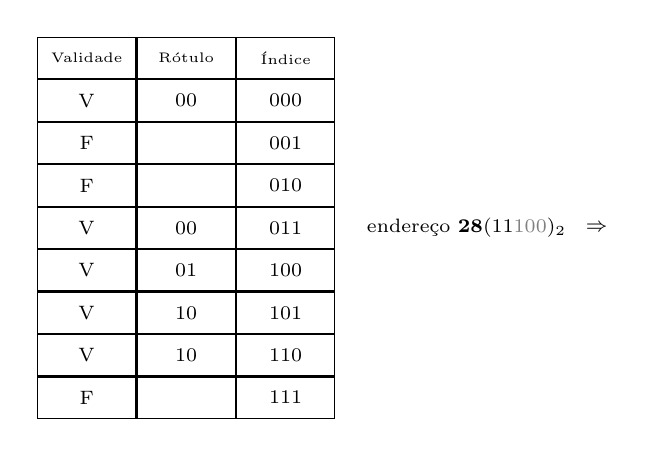
\begin{tikzpicture}[mat/.style={minimum width=1.25cm, minimum
    height=.525cm, draw}, every node/.style={font=\scriptsize}]
  \pgfsetmatrixcolumnsep{1mm}
  \pgfmatrix{rectangle}{center}{mymatrix}
  {\pgfusepath{}}{\pgfpointorigin}{\let\&=\pgfmatrixnextcell}
  {
    \node[mat] {\tiny Validade}; \&[-1mm] \node[mat]{\tiny Rótulo}; \&[-1mm]
    \node[mat] {\tiny Índice}; \\
    \node[mat] {V}; \& \node[mat]{00}; \&  \node[mat] {000}; \\
    \node[mat] {F}; \&  \node[mat]{}; \&  \node[mat] {001}; \\
    \node[mat] {F}; \& \node[mat]{}; \&  \node[mat] {010}; \\
    \node[mat] {V}; \&  \node[mat]{00}; \&  \node[mat] (b0) {011}; \\
    \node[mat] {V}; \& \node[mat]{01}; \&  \node[mat] {100}; \\
    \node[mat] {V}; \&  \node[mat]{10}; \&  \node[mat] {101}; \\
    \node[mat] {V}; \& \node[mat]{10}; \&  \node[mat] {110}; \\
    \node[mat] {F}; \&  \node[mat]{}; \&  \node[mat] {111}; \\
  }

  \node (r0) [right of=b0, xshift=1.25cm] {\lw\ endereço {\bf
      28}(11{\color{gray} 100})$_2$};
  \node (s0) [right of=r0, xshift=.7cm] {$\Rightarrow$};
  \node  [above of=s0] {{\it \miss}};
\end{tikzpicture}
\end{minipage}
\begin{minipage}{.5\textwidth}
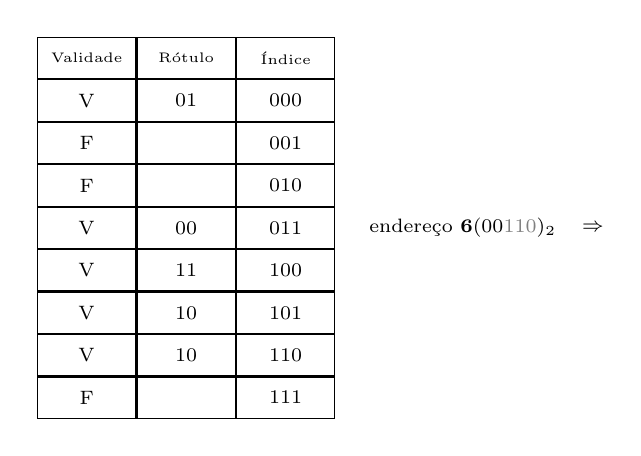
\begin{tikzpicture}[mat/.style={minimum width=1.25cm, minimum
    height=.525cm, draw}, every node/.style={font=\scriptsize}]
  \pgfsetmatrixcolumnsep{1mm}
  \pgfmatrix{rectangle}{center}{mymatrix}
  {\pgfusepath{}}{\pgfpointorigin}{\let\&=\pgfmatrixnextcell}
  {
    \node[mat] {\tiny Validade}; \&[-1mm] \node[mat]{\tiny Rótulo}; \&[-1mm]
    \node[mat] {\tiny Índice}; \\
    \node[mat] {V}; \& \node[mat]{01}; \&  \node[mat] {000}; \\
    \node[mat] {F}; \&  \node[mat]{}; \&  \node[mat] {001}; \\
    \node[mat] {F}; \& \node[mat]{}; \&  \node[mat] {010}; \\
    \node[mat] {V}; \&  \node[mat]{00}; \&  \node[mat] (b0) {011}; \\
    \node[mat] {V}; \& \node[mat]{11}; \&  \node[mat] {100}; \\
    \node[mat] {V}; \&  \node[mat]{10}; \&  \node[mat] {101}; \\
    \node[mat] {V}; \& \node[mat]{10}; \&  \node[mat] {110}; \\
    \node[mat] {F}; \&  \node[mat]{}; \&  \node[mat] {111}; \\
  }

  \node (r0) [right of=b0, xshift=1.2cm] {\lw\ endereço {\bf 6}(00{\color{gray} 110})$_2$};
  \node (s1) [right of=r0, xshift=.7cm] {$\Rightarrow$};
  \node  [above of=s1] {{\it \miss}};
\end{tikzpicture}
\end{minipage}


\begin{minipage}{.5\textwidth}
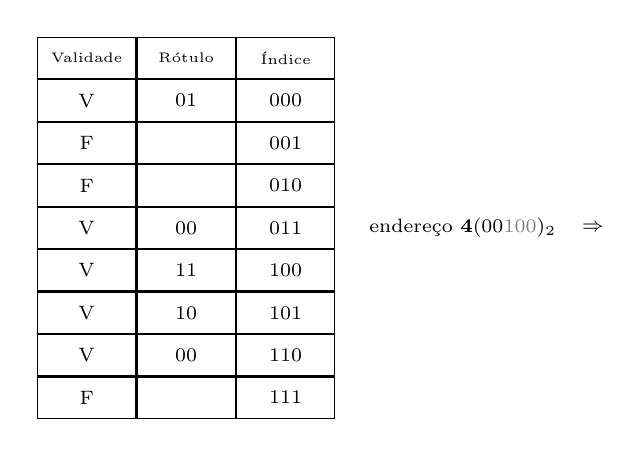
\begin{tikzpicture}[mat/.style={minimum width=1.25cm, minimum
    height=.525cm, draw}, every node/.style={font=\scriptsize}]
  \pgfsetmatrixcolumnsep{1mm}
  \pgfmatrix{rectangle}{center}{mymatrix}
  {\pgfusepath{}}{\pgfpointorigin}{\let\&=\pgfmatrixnextcell}
  {
    \node[mat] {\tiny Validade}; \&[-1mm] \node[mat]{\tiny Rótulo}; \&[-1mm]
    \node[mat] {\tiny Índice}; \\
    \node[mat] {V}; \& \node[mat]{01}; \&  \node[mat] {000}; \\
    \node[mat] {F}; \&  \node[mat]{}; \&  \node[mat] {001}; \\
    \node[mat] {F}; \& \node[mat]{}; \&  \node[mat] {010}; \\
    \node[mat] {V}; \&  \node[mat]{00}; \&  \node[mat] (b0) {011}; \\
    \node[mat] {V}; \& \node[mat]{11}; \&  \node[mat] {100}; \\
    \node[mat] {V}; \&  \node[mat]{10}; \&  \node[mat] {101}; \\
    \node[mat] {V}; \& \node[mat]{00}; \&  \node[mat] {110}; \\
    \node[mat] {F}; \&  \node[mat]{}; \&  \node[mat] {111}; \\
  }

  \node (r0) [right of=b0, xshift=1.2cm] {\lw\ endereço {\bf 4}(00{\color{gray} 100})$_2$};
  \node (s1) [right of=r0, xshift=.7cm] {$\Rightarrow$};
  \node  [above of=s1] {{\it \miss}};
\end{tikzpicture}
\end{minipage}
\begin{minipage}{.5\textwidth}
\begin{tikzpicture}[mat/.style={minimum width=1.25cm, minimum
    height=.525cm, draw}, every node/.style={font=\scriptsize}]
  \pgfsetmatrixcolumnsep{1mm}
  \pgfmatrix{rectangle}{center}{mymatrix}
  {\pgfusepath{}}{\pgfpointorigin}{\let\&=\pgfmatrixnextcell}
  {
    \node[mat] {\tiny Validade}; \&[-1mm] \node[mat]{\tiny Rótulo}; \&[-1mm]
    \node[mat] {\tiny Índice}; \\
    \node[mat] {V}; \& \node[mat]{01}; \&  \node[mat] {000}; \\
    \node[mat] {F}; \&  \node[mat]{}; \&  \node[mat] {001}; \\
    \node[mat] {F}; \& \node[mat]{}; \&  \node[mat] {010}; \\
    \node[mat] {V}; \&  \node[mat]{00}; \&  \node[mat] (b0) {011}; \\
    \node[mat] {V}; \& \node[mat]{00}; \&  \node[mat] {100}; \\
    \node[mat] {V}; \&  \node[mat]{10}; \&  \node[mat] {101}; \\
    \node[mat] {V}; \& \node[mat]{00}; \&  \node[mat] {110}; \\
    \node[mat] {F}; \&  \node[mat]{}; \&  \node[mat] {111}; \\
  }

%  \node (r0) [right of=b0, xshift=1.2cm] {\lw\ endereço {\bf 21}(10{\color{gray} 101})$_2$};
  \node (s1) [right of=r0, xshift=.7cm] {$\Updownarrow$};
  \node  [above of=s1] {{\it EXIT}};
\end{tikzpicture}
\end{minipage}


\bigskip

Taxa de {\bf ausência} de endereços na cache (SRAM) ({\em cache miss}) =
${13 \over 17} * 100 = 76,47\%$ \\

Taxa de {\bf presença} de endereços na cache (SRAM) ({\em cache hit}) = ${4
  \over 17} * 100 = 23,53\%$

\newpage
\subsubsection*{Mapeamento associativo em 2 vias utilizando LRU como
  algoritmo de reposição}

\setcounter{themiss}{0}
\setcounter{thehit}{0}
\def\tdist{8cm}

\begin{tabbing}
  \hspace{3.6cm}\=\cache{\Lambda}{\Lambda}{\Lambda}{\Lambda}, \hspace{3cm}\= $\L\R$
\hspace{.75cm}\\
{\bf 0\ \ } $\Rightarrow$ \miss\>\cache{0,1}{\Lambda}{\Lambda}{\Lambda},\>$\L 0\R$ \\
{\bf 16} $\Rightarrow$ \miss\>\cache{0,1}{\Lambda}{16,17}{\Lambda}, \>$\L\L0\R,\L16\R\R$\\
{\bf 8\ \ }$\Rightarrow$ \miss\>\cache{0,1}{8,9}{16,17}{\Lambda}, \>$\L\L8,0\R, \L16\R\R$\\
{\bf 0\ \ }$\Rightarrow$ \HIT \> \cache{0,1}{8,9}{16,17}{\Lambda},\> $\L\L0,8\R, \L16\R\R$\\
{\bf 0\ \ }$\Rightarrow$ \HIT \> \cache{0,1}{8,9}{16,17}{\Lambda}, \>$\L\L0,8\R, \L16\R\R$\\
{\bf 4\ \ }$\Rightarrow$\miss\> \cache{0,1}{4,5}{16,17}{\Lambda},\>$\L\L4,0\R, \L16\R\R$\\
{\bf 3\ \ }$\Rightarrow$\miss\>\cache{2,3}{4,5}{16,17}{\Lambda},\> $\L\L2,4\R, \L16\R\R$\\
{\bf 12}$\Rightarrow$\miss\>\cache{2,3}{12,13}{16,17}{\Lambda},\> $\L\L12,2\R, \L16\R\R$\\
{\bf 3\ \ }$\Rightarrow$\HIT\>\cache{2,3}{12,13}{16,17}{\Lambda},\>$\L\L2,12\R1~, \L16\R\R$\\
{\bf 11}$\Rightarrow$\miss\>\cache{2,3}{12,13}{16,17}{\Lambda},\> $\L\L12,2\R, \L16\R\R$\\
{\bf 12}$\Rightarrow$\HIT\>\cache{10,11}{12,13}{16,17}{\Lambda},\>$\L\L10,12\R, \L16\R\R$\\
{\bf 21}$\Rightarrow$\miss\>\cache{10,11}{12,13}{16,17}{20,21},\>$\L\L12,10\R,\L20,16\R\R$\\
{\bf 21}$\Rightarrow$\HIT\>\cache{{10,11}}{12,13}{16,17}{20,21},\>$\L\L12,10\R,\L20,16\R\R$\\
{\bf 22}$\Rightarrow$\miss\>\cache{10,11}{12,13}{22,23}{20,21},\>$\L\L12,10\R, \L22,20\R\R$\\
{\bf 28}$\Rightarrow$\miss\>\cache{10,11}{12,13}{22,23}{28,29},\>$\L\L12,10\R, \L28,22\R\R$\\
{\bf 6\ \ }$\Rightarrow$\miss\>\cache{6,7}{12,13}{22,23}{28,29},\>$\L\L 6,12\R,\L 28,22\R\R$\\
{\bf 4\ \ }$\Rightarrow$\miss\>\cache{{6,7}}{4,5}{22,23}{27,28},\>$\L\L4,6\R, \L28,22\R\R$\\
\end{tabbing}


Taxa de {\bf ausência} de endereços na cache (SRAM) ({\em cache miss}) =
${12 \over 17} * 100 = 70,59\%$ \\

Taxa de {\bf presença} de endereços na cache (SRAM) ({\em cache hit}) = ${5
  \over 17} * 100 = 29,41\%$

\paragraph{Explicação.} Os blocos de memória cache estão agrupados por
tuplas designadas pelo símbolo $\L \R$, sendo que cada bloco contém 2 palavras e cada via
contém dois blocos. Por exemplo, na cache

\begin{center}
  \cache{0,1}{2,3}{16,17}{18,19}
\end{center}

os blocos são:  

\begin{itemize}

\item $0 \rightarrow \L 0,1\R$: contendo as palavras dos endereços $0$
  e $1$;
\item $1 \rightarrow \L 2,3\R$: contendo as palavras dos endereços $2$
  e $3$; 
\item $2 \rightarrow \L 16,17\R$: contendo as palavras dos endereços $16$
  e $17$; 
\item $3 \rightarrow \L 18,19\R$: contendo as palavras dos endereços $18$
  e $19$. 

\end{itemize}

Nas tuplas do canto direito são colocadas as palavras que representam
os blocos inseridos, para que possamos saber qual é o utilizado mais
recentemente. Por exemplo, na requisição do endereço $2$ a tupla
torna-se $\L 2\R$, se o endereço $4$ for requisitado em seguida, a
tupla torna-se $\L 4,2\R$, sendo o endereço $4$ o mais recentemente
utilizado. Se o endereço $8$ for inserido, o último da fila sai, a
tupla fica na forma $\L 8,4\R$, sendo $8$ o mais recentemente usado, e
o $4$ o último utilizado recentemente, que sairá da cache, caso haja
necessidade de substituição.

O símbolo $\Lambda$ (lambda maiúsculo) indica que a cache ou bloco estão vazios.

Os endereços entre $0$ e $15$ são mapeados para a via~$0$, enquanto
que entre $16$ e $31$, o mapeamento é efetuado para a via
$1$. Portanto, se houver um requisição pelo endereço $0$, a tupla
correspondente será

\begin{center}
  \cache{0,1}{\Lambda}{\Lambda}{\Lambda}.
\end{center}

Porém, se o próximo endereço requisitado for $16$, este será colocado
na via~$1$, como mostrado a seguir:

\begin{center}
  \cache{0,1}{\Lambda}{16,17}{\Lambda}.
\end{center}

Se a seguir forem requisitados os endereços $6$ e $21$,
respectivamente, a cache fica completa da seguinte forma:

\begin{center}
  \cache{0,1}{6,7}{16,17}{20,21}.
\end{center}

A divisão das vias, blocos e palavras pode ser esquematizada da seguinte forma:

\begin{tabbing}
 via~0 \= $\equiv \L\L 0,1\R,\L 6,7\R\R$\\
 \>bloco~0 \= $\equiv \L 0,1\R$\\
 \>\>palavra~0 $\equiv 0$\\
 \>\>palavra~1 $\equiv 1$\\
 \>bloco~1 $\equiv \L 6,7\R$\\
\>\>palavra~2 $\equiv 6$\\
 \>\>palavra~3 $\equiv 7$\\
  
via~2 $\equiv \L\L 16,17\R,\L 20,21\R\R$\\
 \>bloco~2 $\equiv \L 16,17\R$\\
\>\>palavra~4 $\equiv 16$\\
 \>\>palavra~5 $\equiv 17$\\
  
\>bloco~3 $\equiv \L 20,21\R$\\
\>\>palavra~6 $\equiv 20$\\
 \>\>palavra~7 $\equiv 21$\\
\end{tabbing}


\newpage
\subsubsection*{Mapeamento associativo em 2 vias utilizando algoritmo aleatório}
\label{2-way:lru}

\setcounter{themiss}{0}
\setcounter{thehit}{0}
\def\tdist{8cm}

\begin{tabbing}
\cache{\Lambda}{\Lambda}{\Lambda}{\Lambda}, \hspace{5cm}\= {\bf 0\ \ } $\Rightarrow$\miss\hspace{1.5cm}\=\\
\cache{0,1}{\Lambda}{\Lambda}{\Lambda},\> {\bf 16} $\Rightarrow$\miss\\
\cache{0,1}{\Lambda}{16,17}{\Lambda}, \>{\bf 8\ \ }$\Rightarrow$\miss\\
\cache{0,1}{8,9}{16,17}{\Lambda}, \>{\bf 0\ \ }$\Rightarrow$ \HIT \\
 \cache{0,1}{8,9}{16,17}{\Lambda},\> {\bf 0\ \ }$\Rightarrow$ \HIT \\
 \cache{0,1}{8,9}{16,17}{\Lambda}, \>{\bf 4\ \ }$\Rightarrow$\miss \>rand(2)=1\\
\cache{0,1}{4,5}{16,17}{\Lambda},\> {\bf 3\ \ }$\Rightarrow$\miss \>rand(2)=0\\
\cache{2,3}{4,5}{16,17}{\Lambda},\> {\bf 12}$\Rightarrow$\miss \>rand(2)=0\\
\cache{12,13}{4,5}{16,17}{\Lambda},\> {\bf 3\ \ }$\Rightarrow$\miss \>rand(2)=0\\
\cache{2,3}{12,13}{16,17}{\Lambda},\>{\bf 11}$\Rightarrow$\miss\>rand(2)=0\\
\cache{10,11}{12,13}{16,17}{\Lambda},\>{\bf 12}$\Rightarrow$\HIT\\
\cache{10,11}{12,13}{16,17}{\Lambda},\> {\bf 21}$\Rightarrow$\miss\\
\cache{10,11}{12,13}{16,17}{20,21},\> {\bf 21}$\Rightarrow$\HIT\\
\cache{{10,11}}{12,13}{16,17}{20,21},\>{\bf 22}$\Rightarrow$\miss\\
\cache{10,11}{12,13}{16,17}{22,23},\> {\bf 28}$\Rightarrow$\miss \>rand(2)=1\\
\cache{10,11}{12,13}{16,17}{27,28},\> {\bf 6\ \ }$\Rightarrow$\miss \>rand(2)=1\\
\cache{10,11}{6,7}{22,23}{27,28},\> {\bf 4\ \ }$\Rightarrow$\miss \>rand(2)=1\\
\cache{10,11}{4,5}{22,23}{27,28}\>{\tt EXIT}\\
\end{tabbing}


Taxa de {\bf ausência} de endereços na cache (SRAM) ({\em cache miss}) =
${13 \over 17} * 100 = 76,47\%$ \\

Taxa de {\bf presença} de endereços na cache (SRAM) ({\em cache hit}) = ${4
  \over 17} * 100 = 23,53\%$


\paragraph{Explicação.} A divisão das vias segue o mesmo esquema do
exercício anterior. A função {\tt rand(2)} corresponde ao gerador de
número aleatórios que gera um número inteiro entre $0$ e $2$ (não
incluindo o $2$), ou seja, gera como resultado $0$ ou $1$. Se o número
gerado for $0$, o primeiro bloco é escolhido, caso contrário, $1$
significa escolher o segundo bloco na via correspondente ao endereço.

O gerador de números aleatórios utilizado foi o disponível no site\\
\url{http://www.random.org/}, com o valor mínimo igual a $0$ e máximo
igual a $1$.

\newpage
\subsubsection*{Sem  mapeamento utilizando LRU como
  algoritmo de reposição}

\setcounter{themiss}{0}
\setcounter{thehit}{0}
\def\tdist{8cm}

\begin{tabbing}
  \hspace{3.6cm}\=\cache{\Lambda}{\Lambda}{\Lambda}{\Lambda}, \hspace{3cm}\= $\L\R$
\hspace{.75cm}\\
{\bf 0\ \ } $\Rightarrow$ \miss\>\cache{0,1}{\Lambda}{\Lambda}{\Lambda},\>$\L 0\R$ \\
{\bf 16} $\Rightarrow$ \miss\>\cache{0,1}{16,17}{\Lambda}{\Lambda},\>$\L 16,0\R$\\
{\bf 8\ \ }$\Rightarrow$ \miss\>\cache{0,1}{16,17}{8,9}{\Lambda},\>$\L 8, 16, 0\R$\\
{\bf 0\ \ }$\Rightarrow$ \HIT \> \cache{0,1}{8,9}{16,17}{\Lambda},\>$\L 0, 8, 16\R$\\
{\bf 0\ \ }$\Rightarrow$ \HIT \> \cache{0,1}{8,9}{16,17}{\Lambda},\>$\L 0, 8, 16\R$\\
{\bf 4\ \ }$\Rightarrow$\miss\> \cache{0,1}{8,9}{16,17}{4,5},\>$\L 4, 0 , 8, 16\R$\\
{\bf 3\ \ }$\Rightarrow$\miss\>\cache{0,1}{8,9}{2,3}{4,5},\>$\L 2, 4, 0, 8\R$\\
{\bf 12}$\Rightarrow$\miss\>\cache{0,1}{12,13}{2,3}{4,5},\> $\L 12, 2, 4, 0\R$\\
{\bf 3\ \ }$\Rightarrow$\HIT\>\cache{0,1}{12,13}{2,3}{4,5},\>$\L 2, 12, 4, 0\R$\\
{\bf 11}$\Rightarrow$\miss\>\cache{10,11}{12,13}{2,3}{4,5},\> $\L 10, 2, 12, 4\R$\\
{\bf 12}$\Rightarrow$\HIT\>\cache{10,11}{12,13}{2,3}{4,5},\> $\L 12, 10, 2, 4\R$\\
{\bf 21}$\Rightarrow$\miss\>\cache{10,11}{12,13}{2,3}{20,21},\> $\L 20, 12, 10, 2\R$\\
{\bf 21}$\Rightarrow$\HIT\>\cache{10,11}{12,13}{2,3}{20,21},\> $\L 20, 12, 10, 2\R$\\
{\bf 22}$\Rightarrow$\miss\>\cache{10,11}{12,13}{22,23}{20,21},\> $\L 22, 20, 12, 10\R$\\
{\bf 28}$\Rightarrow$\miss\>\cache{28,29}{12,13}{22,23}{20,21},\> $\L 28, 22, 20, 12\R$\\
{\bf 6\ \ }$\Rightarrow$\miss\>\cache{28,29}{6,7}{22,23}{20,21},\> $\L 6, 28, 22, 20\R$\\
{\bf 4\ \ }$\Rightarrow$\miss\>\cache{28,29}{6,7}{22,23}{4,5},\> $\L 4, 6, 28, 22\R$\\
\end{tabbing}


Taxa de {\bf ausência} de endereços na cache (SRAM) ({\em cache miss}) =
${12 \over 17} * 100 = 70,59\%$ \\

Taxa de {\bf presença} de endereços na cache (SRAM) ({\em cache hit}) = ${5
  \over 17} * 100 = 29,41\%$

\paragraph{Explicação.} A estrutura sem mapeamento é a mesma do
exercício anterior, com a diferença que agora o endereço requisitado
pode ser colocado em qualquer posição, e a fila de recentemente usados
é única, ao invés de ser dividida em vias como no
exercício~\ref{2-way:lru}. Nota-se que o bloco é representado na fila
sempre pelo endereço par do bloco e que o último da fila é sempre o
bloco a ser sobrescrito.

\newpage
\subsubsection*{Sem mapeamento utilizando algoritmo aleatório}
\label{2-way:lru}

\setcounter{themiss}{0}
\setcounter{thehit}{0}
\def\tdist{8cm}

\begin{tabbing}
\cache{\Lambda}{\Lambda}{\Lambda}{\Lambda}, \hspace{5cm}\= {\bf 0\ \ } $\Rightarrow$\miss\hspace{1.5cm}\=\\
\cache{0,1}{\Lambda}{\Lambda}{\Lambda},\> {\bf 16} $\Rightarrow$\miss\\
\cache{0,1}{16,17}{\Lambda}{\Lambda}, \>{\bf 8\ \ }$\Rightarrow$\miss\\
\cache{0,1}{16,17}{8,9}{\Lambda}, \>{\bf 0\ \ }$\Rightarrow$ \HIT \\
 \cache{0,1}{8,9}{16,17}{\Lambda},\> {\bf 0\ \ }$\Rightarrow$ \HIT \\
 \cache{0,1}{8,9}{16,17}{\Lambda}, \>{\bf 4\ \ }$\Rightarrow$\miss\\
\cache{0,1}{8,9}{16,17}{4,5},\> {\bf 3\ \ }$\Rightarrow$\miss \\
\cache{0,1}{8,9}{16,17}{4,5},\> {\bf 12}$\Rightarrow$\miss \>rand(4)=2\\
\cache{0,1}{8,9}{12,13}{4,5},\> {\bf 3\ \ }$\Rightarrow$\miss \>rand(4)=2\\
\cache{0,1}{8,9}{2,3}{4,5},\>{\bf 11}$\Rightarrow$\miss\>rand(4)=1\\
\cache{0,1}{10,11}{2,3}{4,5},\>{\bf 12}$\Rightarrow$\miss\>rand(4)=2\\
\cache{0,1}{10,11}{12,13}{4,5},\> {\bf 21}$\Rightarrow$\miss\>rand(4)=0\\
\cache{20,21}{12,13}{2,3}{4,5},\> {\bf 21}$\Rightarrow$\HIT\\
\cache{20,21}{12,13}{2,3}{4,5},\>{\bf 22}$\Rightarrow$\miss\>rand(4)=0\\
\cache{22,23}{12,13}{2,3}{4,5},\> {\bf 28}$\Rightarrow$\miss \>rand(4)=3\\
\cache{10,11}{12,13}{16,17}{27,28},\> {\bf 6\ \ }$\Rightarrow$\miss \>rand(4)=0\\
\cache{6,7}{12,13}{16,17}{27,28},\> {\bf 4\ \ }$\Rightarrow$\miss \>rand(4)=1\\
\cache{6,7}{4,5}{16,17}{27,28}\>{\tt EXIT}\\
\end{tabbing}



Taxa de {\bf ausência} de endereços na cache (SRAM) ({\em cache miss}) =
${14 \over 17} * 100 = 82,35\%$ \\

Taxa de {\bf presença} de endereços na cache (SRAM) ({\em cache hit}) = ${3
  \over 17} * 100 = 17,65\%$\\

\paragraph{Explicação.}O gerador de número aleatórios {\tt rand(4)} gera números inteiros
entre 0 e 4 (não incluindo o $4$), pois agora a substituição da
cache pode ser realizada em qualquer um dos blocos de $0$ a $3$. 

A ordem de inserção quando a cache estiver com blocos livres é
arbitrária. Poderia até ser usado o {\tt rand(4)} para saber em qual
bloco escrever o conteúdo do endereço requisitado quando a cache
estiver vazia.

O essencial é entender o método de reposição baseado na aleatoriedade
que não leva em conta a localidade temporal ou espacial, como acontece
com a reposição baseada no algoritmo LRU.


Realize as requisições dos itens $a$ e $b$ separadamente e utilize o
algoritmo LRU e a política de reposição aleatória para trocar o
conteúdo dos blocos na cache. Para a política aleatória, pegue uma
moeda e atribua o valor $0$ ou $1$ para cara ou coroa, correspondendo
à posição do bloco a ser trocado no conjunto.

